\input{estilo}
\newcommand\ix[1]{[\kern0.6pt\var{#1}\kern1.2pt]}
\newcommand\V[1]{\var{V}\textsubscript{\var{i}}\ix{#1}}
\newcommand\pii{\var{p}\textsubscript{\var{i}}}
\begin{document}
\begin{figura}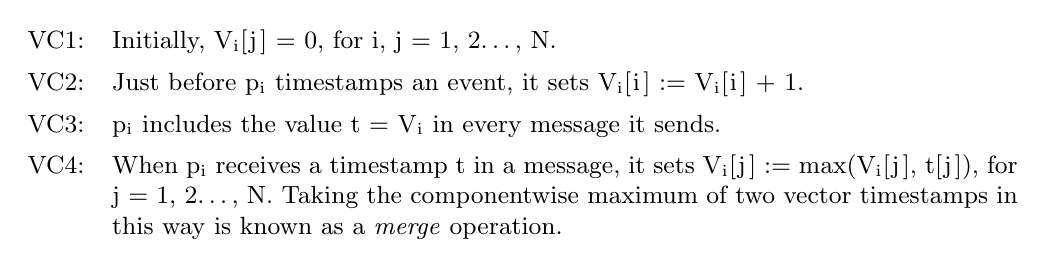
\begin{tikzpicture}
  \node[anchor=north west, font=\small, inner sep=0pt] {%
    \begin{tabular}{@{}l@{\hspace{10pt}}p{11.5cm}@{}}
      VC1: & Initially, \V{j} = 0, for \var{i}, \var{j} = 1, 2…, \var{N}.\\[4pt]
      VC2: & Just before \pii\ timestamps an event, it sets \V{i} := \V{i} + 1.\\[4pt]
      VC3: & \pii\ includes the value \var{t} = \var{V}\textsubscript{\var{i}} in every message it sends.\\[4pt]
      VC4: & When \pii\ receives a timestamp \var{t} in a message, it sets
             \V{j} := max(\V{j}, \var{t}\ix{j}), for \var{j} = 1, 2…, \var{N}. Taking the
             componentwise maximum of two vector timestamps in this way is known as a
             \textit{merge} operation.
    \end{tabular}};
\end{tikzpicture}\end{figura}
\end{document}
